\documentclass[10pt]{article}

\def\Type{LessonCaelan}
\def\TypeNum{Lesson 11}
\def\TypeTitle{Local Extrema \& First Derivative Test }
\def\Semester{Fall 2021} %Not Used 
\def\Course{MATH 1190 \& 1210}
\def\Targets{ {\bf\color{RedOrange}A1}, {\bf\color{RedOrange}A2} }

\usepackage{preambleDJ}

%\usepackage{ragged2e}


%%%%%%%%%%%% BEGIN DOCUMENT %%%%%%%%%%%%%%%
%%%%%%%%%%%% BEGIN DOCUMENT %%%%%%%%%%%%%%%
%%%%%%%%%%%% BEGIN DOCUMENT %%%%%%%%%%%%%%%
%%%%%%%%%%%% BEGIN DOCUMENT %%%%%%%%%%%%%%%
%%%%%%%%%%%% BEGIN DOCUMENT %%%%%%%%%%%%%%%



\begin{document}

\pagestyle{otherpages}
\thispagestyle{firstpage}
\vs{.6}

\textbf{Intended Learning Outcomes}
After this lesson, you will be able to 

\begin{itemize}
    \item Identify increasing/decreasing intervals and critical numbers of a function from given graph or formula. (\target{A1})
    \item Represent concepts such as derivatives, local extrema, and critical number graphically. (\target{A1})
    \item Apply the First Derivative Test to determine the local extrema of a function graphically and algebraically. (\target{A2})
\end{itemize}

\vspace{-0.5cm}

\hrulefill\\
In this activity, we establish a means of finding local extreme values (also called relative extreme values) of a function using properties of the derivative. First, review some key ideas from the online class prep activity to prepare yourself for the important ideas of the lesson.\\

{\bf \textcolor{blue}{Warm-up Exercise 1.}}\ltrm{\color{RedOrange}A1}  Respond to the prompt below.
%
 \important{Definition: Critical Number}
    {
    A {\em critical number} is  a number $c$ in the \blue{\it domain} of $f$ where either
  \begin{center} \blue{ $f'(c) = 0$} \quad\quad\quad or \quad\quad\quad \blue{$f'(c) \qquad DNE$} \end{center}
    }
    
    {\bf TRUE or FALSE?} $\displaystyle f(x)=\frac1x$ has exactly 1 critical number. \hfill (circle one): \hfill {\bf TRUE} \hfill {\bf FALSE}\\ Explain your decision.
    
\vs{1.25}
 
{\bf \color{blue} Mini-lecture: } Connecting the sign of $f'$ to the locations of local extrema.\\
\mpageT{.33}{.8}[\hs{.1}]{
%
\includegraphics[width=0.95\textwidth]{images/1st derivative test.PNG}
\begin{flushleft}
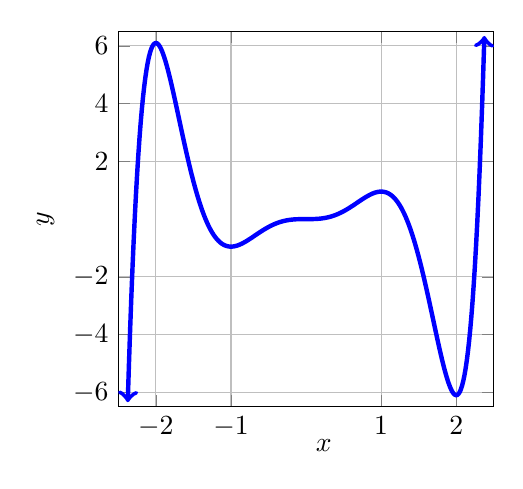
\begin{tikzpicture}
    \begin{axis}[
    	x label style={anchor=west},
            xlabel={$x$},
            xtick       = {-2,-1,1,2},
            xticklabels = {$-2$,$-1$,$1$,$2$},
            y label style={anchor=south},
            ylabel={$y$},
            ytick       = {-6,-4,-2,2,4,6},
            yticklabels = {$-6$,$-4$,$-2$,$2$,$4$,$6$},
            samples     = 320,
            domain      = -2.5:2.5,
            restrict y to domain=-6.5:6.5,
            xmin = -2.5, xmax = 2.5,
            ymin = -6.5, ymax = 6.5,
            width=2.5in, height=2.5in,
            grid=both, grid style=solid
          ]
    \addplot[domain=-2.5:2.5, blue, ultra thick, mark=none, <->]{2*(x^7/7-x^5+4/3*x^3)};
    \end{axis}
\end{tikzpicture}
\end{flushleft}
\itemNIN{
\item Highlight  graph where increasing.
\item Highlight  graph where decreasing
\item Place a point on the graph at each critical number.
}
}{
 \important{First Derivative Test}
	{
	Suppose that $c$ is a \blue{\em critical number} of a continuous function $f$.
			\enumA{
			\mpageT{.6}{.4}{
			\item If $f'$ changes from \blue{(+)} to \blue{(-)} at $c$, then $f$ has:\vs{.75}
			}{
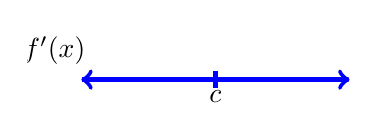
\begin{tikzpicture}
    \begin{axis}[
    	axis x line=none,
	            axis y line=none,
		x label style={anchor=west},
            xlabel={},
            xtick       = {0},
            xticklabels = {$c$},
            y label style={anchor=south},
            ylabel={},
            ytick       = {-6,-4,-2,2,4,6},
            yticklabels = {$-6$,$-4$,$-2$,$2$,$4$,$6$},
            samples     = 320,
            domain      = -2.5:2.5,
            restrict y to domain=-6.5:6.5,
            xmin = -3.5, xmax = 3.5,
            ymin = -6.5, ymax = 6.5,
            width=2.5in, height=2.5in,
            grid=none, grid style=solid
          ]
    \addplot[domain=-2.5:2.5, blue, ultra thick, mark=none, <->]{0)};
   \draw (-3,1) node{$\Large f^{\prime}(x)$};
   \draw[ultra thick, blue] (0,.3)--(0,-.3);
      \draw (0,-.6) node{$c$};
    \end{axis}
\end{tikzpicture}
			}
			\mpageT{.6}{.4}{
			\item If $f'$ changes from \blue{(-)} to \blue{(+)} at $c$, then $f$ has:\vs{.75}
			}{
			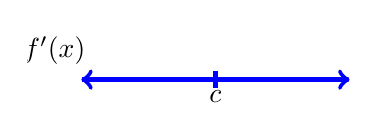
\begin{tikzpicture}
    \begin{axis}[
    	axis x line=none,
	            axis y line=none,
		x label style={anchor=west},
            xlabel={},
            xtick       = {0},
            xticklabels = {$c$},
            y label style={anchor=south},
            ylabel={},
            ytick       = {-6,-4,-2,2,4,6},
            yticklabels = {$-6$,$-4$,$-2$,$2$,$4$,$6$},
            samples     = 320,
            domain      = -2.5:2.5,
            restrict y to domain=-6.5:6.5,
            xmin = -3.5, xmax = 3.5,
            ymin = -6.5, ymax = 6.5,
            width=2.5in, height=2.5in,
            grid=none, grid style=solid
          ]
    \addplot[domain=-2.5:2.5, blue, ultra thick, mark=none, <->]{0)};
   \draw (-3,1) node{$\Large f^{\prime}(x)$};
   \draw[ultra thick, blue] (0,.3)--(0,-.3);
      \draw (0,-.6) node{$c$};
    \end{axis}
\end{tikzpicture}
}
\mpageT{.6}{.4}{
			\item If $f'$ does not change sign at $c$, then $f$ has:\vs{.75}
			}{
			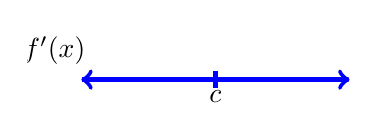
\begin{tikzpicture}
    \begin{axis}[
    	axis x line=none,
	            axis y line=none,
		x label style={anchor=west},
            xlabel={},
            xtick       = {0},
            xticklabels = {$c$},
            y label style={anchor=south},
            ylabel={},
            ytick       = {-6,-4,-2,2,4,6},
            yticklabels = {$-6$,$-4$,$-2$,$2$,$4$,$6$},
            samples     = 320,
            domain      = -2.5:2.5,
            restrict y to domain=-6.5:6.5,
            xmin = -3.5, xmax = 3.5,
            ymin = -6.5, ymax = 6.5,
            width=2.5in, height=2.5in,
            grid=none, grid style=solid
          ]
    \addplot[domain=-2.5:2.5, blue, ultra thick, mark=none, <->]{0)};
   \draw (-3,1) node{$\Large f^{\prime}(x)$};
   \draw[ultra thick, blue] (0,.3)--(0,-.3);
      \draw (0,-.6) node{$c$};
    \end{axis}
\end{tikzpicture}
}
			}
	}
}

\newpage
 
 {\bf \textcolor{blue}{Warm-up Exercise 2}}\ltrm{\target{A1}}  Sketch the graph of a function $f$ satisfying the following:\\
 
\begin{minipage}[t]{0.6\textwidth}
 \begin{itemize}
 \item $f'(2)=0$ and $f(2)$ is a local/relative minimum
 \item $f'(4)=0$ and $f(4)$ is neither a maximum nor a minimum
 \item $f'(6)$ DNE and $f(6)$ is a local/relative maximum
 \end{itemize}
 \end{minipage}
 \hfill
 \begin{minipage}[t]{0.38\textwidth}
 \vspace{-0.2in}
 \begin{center}
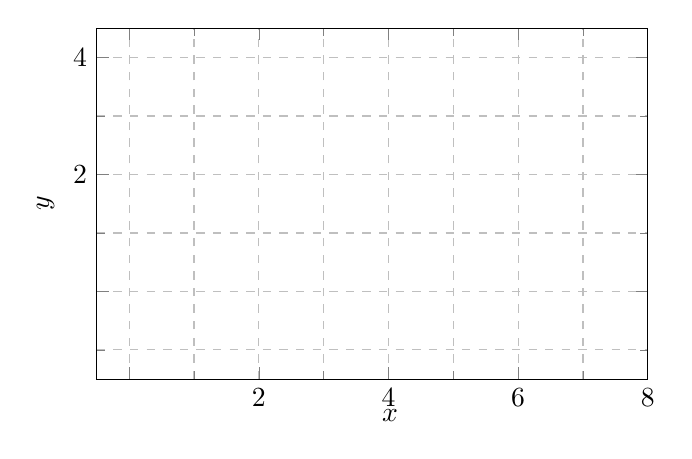
\begin{tikzpicture}s
    \begin{axis}[scale=2,
    	x label style={anchor=west},
            xlabel={$x$},
            xtick       = {0,2,4,6,8},
            xticklabels = {,$2$,$4$,$6$,$8$},
            y label style={anchor=south},
            ylabel={$y$},
            ytick       = {-2,0,2,4},
            yticklabels = {,,$2$,$4$},
            minor tick num=1,
            samples     = 320,
            domain      = -.5:8,
            restrict y to domain=0:5,
            xmin = -.5, xmax = 8,
            ymin = -1.5, ymax = 4.5,
            width=2in, height=1.5in,
            grid=both, grid style=dashed
          ]
%    \addplot[domain=0:5, red, ultra thick, mark=none, -]{1/18*(x-2)^2*(3*x^2-28*x+68)};
%        \addplot[domain=5:6, red, ultra thick, mark=none, -]{2*x-17/2};
%                \addplot[domain=6:8, red, ultra thick, mark=none, -]{-2*x+31/2};
    \end{axis}
\end{tikzpicture}
 \end{center}
 \end{minipage}
 
 \vspace{0.5in}

%\vs{.5}
%{\em Practical Tip: Sign Line (i.e. Number Line)}\vs{.3}\\
%\begin{center}
%\begin{tikzpicture}
%    \begin{axis}[
%    	axis x line=none,
%	            axis y line=none,
%		x label style={anchor=west},
%            xlabel={},
%            xtick       = {-2,-1,1,2},
%            xticklabels = {$-2$,$-1$,$1$,$2$},
%            y label style={anchor=south},
%            ylabel={},
%            ytick       = {-6,-4,-2,2,4,6},
%            yticklabels = {$-6$,$-4$,$-2$,$2$,$4$,$6$},
%            samples     = 320,
%            domain      = -2.5:2.5,
%            restrict y to domain=-6.5:6.5,
%            xmin = -3.5, xmax = 3.5,
%            ymin = -6.5, ymax = 6.5,
%            width=5in, height=2.5in,
%            grid=none, grid style=solid
%          ]
%    \addplot[domain=-2.5:2.5, blue, ultra thick, mark=none, <->]{0)};
%   \draw (-3,1) node{$\Large f^{\prime}(x)$};
%    \end{axis}
%\end{tikzpicture}
%\end{center}


\example Let $g(x)=x-\ln(x^2+1)$.
%
\begin{enumerate}
\item[(a)]\ltrm{\target{A1}} Find the critical numbers of $g$.

\vs{3}

\item[(b)]\ltrm{\color{RedOrange}\bf A1} Find the intervals where $g$ is increasing or decreasing. {\em Hint:} Creating a sign line will probably be helpful.


\vs{2}

\item[(c)]\ltrm{\color{RedOrange}\bf A2} At which critical number(s) does $g$ attain a local extreme value(s)? Explicitly cite a relevant test in your response.



\end{enumerate}

\newpage

\exercise Let $f(x)=\dfrac{x}{x^2+1}$.
\begin{enumerate}
\item[(a)] \ltrm{\color{RedOrange}\bf A1} Find the intervals where $f$ is increasing or decreasing. Draw a number line to depict your answer, and record your final answer using interval notation. \\
\vs{5.5}


\item[(b)] \ltrm{\color{RedOrange}\bf A2} Find the local maximum \& local minimum points of $f$. Explicitly cite a relevant test in your response. \\


\end{enumerate}

\newpage
{\bf Note:} The next problem will test your conceptual understanding of what it means for a function to increase or decrease, as well as of the definition of a critical number. A variation of this problem appeared on an exam during the Fall 2023 semester.\\
\exercise{{\bf\color{RedOrange}A1}}  What would the {\em critical numbers} of the function $f$ be if...
\enumA{
\mpageT{.55}{.45}{
\vs{.3}
%\enumA{
\item  the curve pictured to the right is the graph of $f$? \vs{.75}
%}
}{
\begin{flushright}
    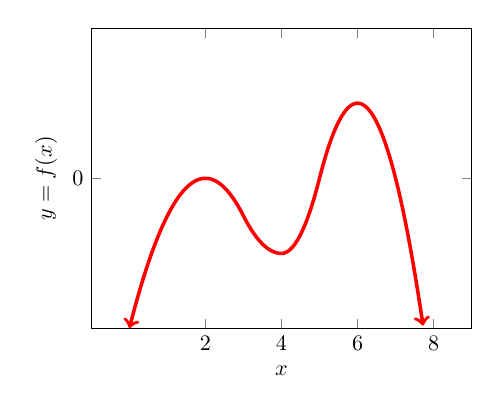
\begin{tikzpicture}[scale=.8]
          \begin{axis}[
            xlabel={$x$},
            ylabel={$y=f(x)$},
            %grid = major,
            xtick       = {2,4,6,8},
            xticklabels = {$2$,$4$,$6$,$8$},
            ytick       = {0},
            yticklabels = {$0$},
            samples     = 320,
            domain      = -1:9,
            restrict y to domain=-4:4,
            xmin = -1, xmax = 9,
            ymin = -4, ymax = 4,
            height=2.5in, width=3in
          ]
          % old version of the curve
          %
          %\addplot[domain=-1:9, purple, ultra thick, mark=none] {-1/10*(x-1)*(x-4)^2*(x-7)};
          %
          %new version of the curve in pieces
          %
          \addplot[domain=-1:3, ultra thick, red,<-] {-(x-2)^2};
          \addplot[domain=3:4, ultra thick, red] {(x-4)^2-2};
          \addplot[domain=4:5, ultra thick, red] {2*(x-4)^2-2};
          \addplot[domain=5:9, ultra thick, red,->] {-2*(x-6)^2+2};
          %
        \end{axis}
    \end{tikzpicture}
\end{flushright}
}

\mpageT{.55}{.45}{\vs{.3}
%\enumA{\setItemnumber{2}
\item the curve pictured to the right is the graph of $f'$? \vs{.75}
%}
}{
\begin{flushright}
    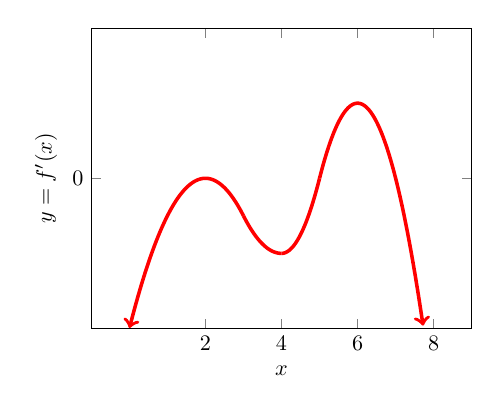
\begin{tikzpicture}[scale=.8]
          \begin{axis}[
            xlabel={$x$},
            ylabel={$y=f^{\prime}(x)$},
            %grid = major,
            xtick       = {2,4,6,8},
            xticklabels = {$2$,$4$,$6$,$8$},
            ytick       = {0},
            yticklabels = {$0$},
            samples     = 320,
            domain      = -1:9,
            restrict y to domain=-4:4,
            xmin = -1, xmax = 9,
            ymin = -4, ymax = 4,
            height=2.5in, width=3in
          ]
          % old version of the curve
          %
          %\addplot[domain=-1:9, purple, ultra thick, mark=none] {-1/10*(x-1)*(x-4)^2*(x-7)};
          %
          %new version of the curve in pieces
          %
          \addplot[domain=-1:3, ultra thick, red,<-] {-(x-2)^2};
          \addplot[domain=3:4, ultra thick, red] {(x-4)^2-2};
          \addplot[domain=4:5, ultra thick, red] {2*(x-4)^2-2};
          \addplot[domain=5:9, ultra thick, red,->] {-2*(x-6)^2+2};
          %
        \end{axis}
    \end{tikzpicture}
\end{flushright}
}
}
\exercise{{\bf\color{RedOrange}A1}}  On which intervals would the function $f$ be {\it decreasing} if...
\enum{
\mpageT{.55}{.45}{
\vs{.3}
\item the curve pictured to the right is the graph of $f$?
}{
\begin{flushright}
    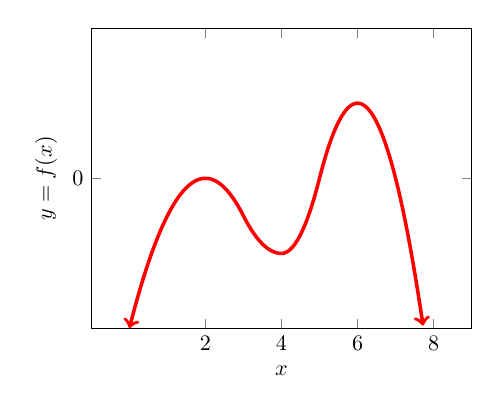
\begin{tikzpicture}[scale=.8]
          \begin{axis}[
            xlabel={$x$},
            ylabel={$y=f(x)$},
            %grid = major,
            xtick       = {2,4,6,8},
            xticklabels = {$2$,$4$,$6$,$8$},
            ytick       = {0},
            yticklabels = {$0$},
            samples     = 320,
            domain      = -1:9,
            restrict y to domain=-4:4,
            xmin = -1, xmax = 9,
            ymin = -4, ymax = 4,
            height=2.5in, width=3in
          ]
          % old version of the curve
          %
          %\addplot[domain=-1:9, purple, ultra thick, mark=none] {-1/10*(x-1)*(x-4)^2*(x-7)};
          %
          %new version of the curve in pieces
          %
          \addplot[domain=-1:3, ultra thick, red,<-] {-(x-2)^2};
          \addplot[domain=3:4, ultra thick, red] {(x-4)^2-2};
          \addplot[domain=4:5, ultra thick, red] {2*(x-4)^2-2};
          \addplot[domain=5:9, ultra thick, red,->] {-2*(x-6)^2+2};
          %
        \end{axis}
    \end{tikzpicture}
\end{flushright}
}
\mpageT{.55}{.45}{
\vs{.3}
\item the curve pictured to the right is the graph of $f'$?
}{
\begin{flushright}
    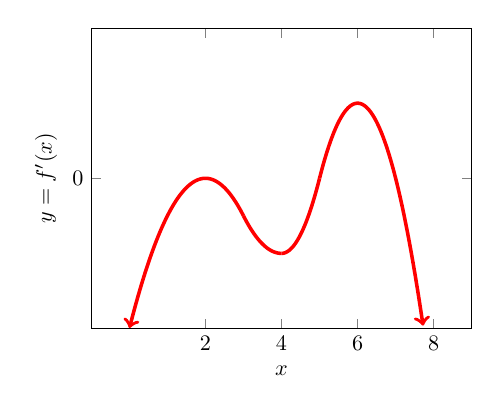
\begin{tikzpicture}[scale=.8]
          \begin{axis}[
            xlabel={$x$},
            ylabel={$y=f^{\prime}(x)$},
            %grid = major,
            xtick       = {2,4,6,8},
            xticklabels = {$2$,$4$,$6$,$8$},
            ytick       = {0},
            yticklabels = {$0$},
            samples     = 320,
            domain      = -1:9,
            restrict y to domain=-4:4,
            xmin = -1, xmax = 9,
            ymin = -4, ymax = 4,
            height=2.5in, width=3in
          ]
          % old version of the curve
          %
          %\addplot[domain=-1:9, purple, ultra thick, mark=none] {-1/10*(x-1)*(x-4)^2*(x-7)};
          %
          %new version of the curve in pieces
          %
          \addplot[domain=-1:3, ultra thick, red,<-] {-(x-2)^2};
          \addplot[domain=3:4, ultra thick, red] {(x-4)^2-2};
          \addplot[domain=4:5, ultra thick, red] {2*(x-4)^2-2};
          \addplot[domain=5:9, ultra thick, red,->] {-2*(x-6)^2+2};
          %
        \end{axis}
    \end{tikzpicture}
\end{flushright}
}
}




\newpage
{\bf Note:} The next problem will test your comprehension of Warm-up Exercise 1 and the Chain Rule.\\

{\bf\color{blue} Extra Practice 1.}\ltrm{\color{RedOrange}A1} Find all critical numbers of $f(x)=\sqrt[3]{x^2-4x}$.

\vs{3}





{\bf Note:} The next 2 exercises make use of all the information in this worksheet and the associated pre-class assignment. The goal is for you to continue to fluently apply the definition of a critical number, to find \& interpret the sign of the first derivative as it relates to whether a function is increasing or decreasing, and to use the First Derivative Test to classify critical numbers.\\

{\bf\color{blue} Extra Practice 2.} Let $f(x)=\ln(x^2-2x+1)$. 
\enumA{
\item \ltrm{\color{RedOrange}A1} Find all critical numbers of $f$.
    \vfill
    
\item \ltrm{\color{RedOrange}A1} Find the intervals on which $f$ is increasing \& the intervals on which $f$ is decreasing.
    \vfill
    \vfill

\item \ltrm{\color{RedOrange}A2} At which $x$-values does $f$ have local maximum values? At which $x$-values does $f$ have local minimum values? Explain.
    \vfill
}

%%%%%%%%%
\newpage%
%%%%%%%%%

{\bf\color{blue} Extra Practice 3.} Let $f(x)=\dfrac15x^5-\dfrac53x^3+4x$.
\enumA{
\item \ltrm{\color{RedOrange}A1} Find the critical numbers of $f$.
    \vfill
\item \ltrm{\color{RedOrange}A1} Find the intervals where $f$ is increasing or decreasing.
    \vfill
    \vfill
\item \ltrm{\color{RedOrange}A2} At which critical number(s) does $f$ attain local extrema? Explain.
    \vfill
    \vfill
}

\end{document}


